\tasknumber{2018}{15} Дан $\triangle OAB.$ $O(0;0),$ $A(2;2),$ $B(x;2).$ Найдите координаты точки $B$, если площадь треугольника $OAB=4$. \\
\begin{figure}[h]
	\centering
	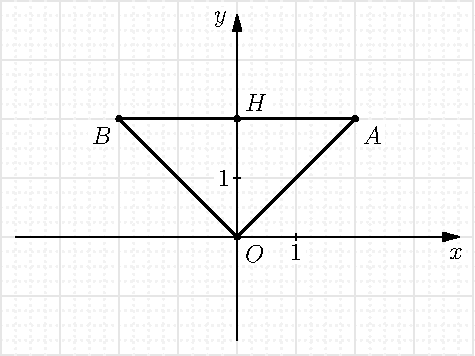
\includegraphics[scale = 1]{pic19.pdf}
\end{figure}
\Solution
Поставим на координатной плоскости точки $O$ и $A$ и точку $B$ с ординатой $2$.\\
Высота $OH$, проведенная к стороне $OB$ -- фиксированная и равна двум клеткам, тогда площадь $\triangle OAB$ равна
\begin{center}$
S=\dfrac12\cdot2\cdot|x-2|=4 \Leftrightarrow |x-2|=4 \Leftrightarrow \left[ \begin{array}{l} x=-2,\\x=6.
\end{array}\right.$\\
\end{center}
\Answer{$(-2;2), (6;2)$}

